
\chapter{$k$-Analytic Spaces}

To develop a satisfactory geometric theory of analytic spaces, we start by developing the corresponding algebraic theory before using this to define the basic building blocks of analytic spaces. The material in this chapter primarily follows \parencite{berk1} and \parencite{temk}.

\section{$k$-Affinoid Spectra}

Let $A$ be a commutative ring with unity.
A \textit{seminorm} (resp. \textit{non-Archimedean seminorm}) on $A$ is a function $|\cdot|: A \to \mathbb{R}_{\geq 0}$ such that for all $f, g \in k$ the following hold:
\begin{enumerate}
    \item $|0| = 0$ and $|1| = 1$;
    \item $|f \cdot g| \leq |f| \cdot |g|$;
    \item $|f - g| \leq |f| + |g|$ (resp. $|f - g| \leq \max \{|f|, |g|\}$).
\end{enumerate}

If we have that $|f| = 0$ if and only if $f = 0$, then the seminorm is called a \textit{norm}.
Note that we assume any norm to be submultiplicative.
If for all $f, g \in k$, $|f \cdot g| = |f| \cdot |g|$, then the norm is said to be multiplicative; a multiplicative norm is an \textit{absolute value}. 
Then, any norm on $A$ induces a topology and hence we may take the completion of $A$ with respect to the given norm.
For a normed ring $(A, |\cdot|)$, we define:
\begin{align*}
A^{\circ} & := \{ a \in A \; | \; |a| \leq 1\} \\
A^{\circ\circ} & := \{ a \in A \; | \; |a| < 1\}    
\end{align*}
The \textit{residue ring} $\tilde A$ is then given by $A^{\circ}/A^{\circ\circ}$.
A complete normed ring is called a \textit{Banach ring}. 
Given a Banach ring $\banr$ with norm $\norm$, we say that a seminorm $\snorm$ on $\banr$ is \textit{bounded} if for all $f \in \banr$, $|f| \leq C||f||$ for some constant $C$. 
If the seminorm is multiplicative, then we may take $C = 1$.
A morphism of Banach rings $\phi: (\banr, \norm_\banr) \to (\banb, \norm_\banb)$ is a homomorphism of the rings which is bounded in the sense that $||\phi(a)||_{\banb} \leq C \cdot ||a||_{\banr}$, for any $a \in \banr$ and some constant $C$. For our purposes, it suffices to consider only Banach $k$-algebras.

For any $r = (r_1, \dots, r_n) \in \RR_{\geq 0}^n, a = (a_1, \dots, a_n) \in k^n$, we define the Banach $k$-algebra:
\begin{align*}
& k\{r^{-1}({T} -  {a})\} = k\{r_1^{-1}(T_1 - a_1), \dots, r_n^{-1}(T_n - a_n)\} \\ & := \left\{
    f = \sum\limits_{|\alpha| \geq 0} c_{\alpha}( {T} -  {a})^{\alpha} \; \vert \;
        c_{\alpha} \in k \; \text{and} \; |c_{\alpha}| r^{|\alpha|} \to 0 \; \text{as} \; |\alpha| \to \infty
\right\}
\end{align*}

The norm on this algebra is given by $||f|| := \max_{\alpha} |c_{\alpha}|  {r}^{|\alpha|}$. Although not immediate, the following lemma describes some well-known properties of the norm.

\begin{lemma}\label{tatealgnorm}\parencite[\S 6.1.5]{bgr}
    The norm $||\cdot||$ on $k\{ {r}^{-1}( {T} -  {a})\}$ is multiplicative, and hence an absolute value. Furthermore, when $k$ is algebraically closed, for any $f \in k\{r^{-1}(T - a)\}$ we have that:
    \[
    \max_{\alpha} \{ |c_{\alpha}|  {r}^{|\alpha|} \} = \sup_{z \in \overline{B}(a, r)} |f(z)|
    \]
    where $\overline{B}(a, r) \subset k^n$ denotes the closed ball of radius $r$ centered at $a$.
\end{lemma}

The algebras described are the analytic counterpart to polynomial rings in $n$ variables over $k$ - they additionally capture the notion of convergence of a power series on a polydisk centered at $a$ with radius $r$. This analogy extends to define a corresponding notion of finitely generated algebras.

For a closed ideal $I$ of a Banach ring $\banr$ with norm $||\cdot||$, the quotient $\banr/I$ has an induced norm, called the residue norm, given by $|f + I| = \inf_{h \in I} ||f + h||$. 
Two norms are equivalent if they are both bounded by each other. We say a map of Banach rings $\phi: \banr \to \mathscr{B}$ is admissible if the residue norm on $\banr/\ker \phi$ is equivalent to the norm on $\mathscr{B}$ restricted to $\operatorname{im} \phi$. 

\begin{defn}\parencite[\S 2.1]{berk1}
    A \textit{$k$-affinoid algebra} $\banr$ is a Banach $k$-algebra such that there is an admissible surjective homomorphism of Banach algebras $k\{ {r}^{-1} {T}\} \to \banr$, for some $ {r} \in \RR_{> 0}^n$ and some $n \geq 0$.
\end{defn}

Hence, the above definition means that we may identify, as Banach $k$-algebras, a $k$-affinoid algebra with a quotient of $k\{r^{-1}T\}$. 
A $k$-affinoid algebra $\banr$ is Noetherian and all ideals are closed \parencite[Prop. 2.1.3]{berk1}, so it makes sense to talk about quotients $\banr/I$ where $I$ is a necessarily finitely generated ideal of $\banr$.

Next, we introduce an analogue of the $\spec$ construction in the form of the Berkovich spectrum of a Banach ring.

\begin{defn}\parencite[\S 1.2]{berk1}
    Let $(\banr, \norm)$ be a Banach ring. The Berkovich spectrum $\berkspec{\banr}$ is the set of
    all multiplicative seminorms on $\banr$, bounded with respect to $\norm$. The topology is the
    weakest such that for all $f \in \banr$, the function $\berkspec{\banr} \to \mathbb{R}_{\geq 0}$ given by $\snormx \mapsto |f|_x$ is continuous.
\end{defn}

We will identify a point $x \in \berkspec{\banr}$ with a seminorm, denoted $\snormx$. 
For a non-zero Banach ring $\banr$, the spectrum $\berkspec{\banr}$ is non-empty, compact and Hausdorff \parencite[Theorem 1.2.1]{berk1}, and when the norm on $\banr$ is non-Archimedean, the points of $\berkspec{\banr}$ are non-Archimedean seminorms.

\begin{example}
    For any field $K$ endowed with a non-Archimedean absolute value $||\cdot||$, the spectrum $\berkspec{K}$ consists of a single point.
    Indeed, taking any element ${\snormx} \in \berkspec{K}$ and $f \in K^{\times}$, we see that $|f|_x \leq ||f||$. But additionally, $|f^{-1}|_x \leq ||f^{-1}||$, which implies by multiplicativity that $||f|| = |f|_x$. 
    Hence the only point of $\berkspec{K}$ is the absolute value on $K$.
\end{example}

\begin{example}
     For all $n > 0$, $ {a} \in k^n$ and $ {r} \in \RR_{> 0}^n$, the \textit{Berkovich closed disk} $E( {a},  {r})$ is defined as 
     \[E( {a},  {r)} = \berkspec{k\{ {r}^{-1}( {T} -  {a})\}}.\] 
     Since the norm $||\cdot||$ on $k\{ {r}^{-1}( {T} -  {a})\}$ is multiplicative, it gives a point of $E( {a},  {r})$ which - by definition of the spectrum - is maximal in the sense that for any other point $\snormx$ and $f \in k\{ {r}^{-1}( {T} -  {a})\}$, we have that $|f|_x \leq ||f||$.
\end{example}

The closed disk admits the following description.

\begin{prop}\label{prop:diskmaxpoint}\parencite[\S 1.4.4]{berk1}
    For all $n > 0$, $ {a} = (a_1, \dots, a_n) \in k^n$ and ${ {r} = (r_1, \dots, r_n) \in \RR_{> 0}^n}$, the closed disk $E( {a},  {r})$ is identified with the set of multiplicative seminorms on $k[T_1, \dots, T_n]$ extending the absolute value on $k$ such that $|T_i - a_i|_x \leq r_i$ for all $1 \leq i \leq n$.
\end{prop}
\begin{proof}
    We may assume by a suitable change of coordinates that $ {a} =  {0} \in k^n$.
    Fix a point $x \in E(0, r)$. Then any such point defines a multiplicative seminorm on $k[T_1, \dots, T_n]$ by 
    restricting along the inclusion $k[T_1, \dots, T_n] \subset k\{r^{-1}T\}$. 
    The fact that $\snormx$ is bounded by the norm on $k\{r^{-1}T\}$ immediately implies that the seminorm extends the absolute value on $k$ and that $|T_i|_x \leq r_i$ for all $1 \leq i \leq n$.
    
    Conversely, fix a seminorm $\snormx$ as in the statement of the theorem, and assume $|T|_x \leq r$. For an element
    \[
        f = \sum\limits_{|\alpha| = 0}^{\infty} c_\alpha T^\alpha \in \tatealgr
    \]
    we define the sequence $(f_n)_{n \in \NN}$, where for any $n \in \NN$,
    \[
        f_n := \sum\limits_{|\alpha| = 0}^{n} c_{\alpha} T^{\alpha} \in k[T_1, \dots, T_n]
    \]
    and subsequently define a map on $k\{r^{-1}T\}$ sending $f \mapsto \lim_{n \to \infty} |f_n|_x$.
    
    To see that this limit exists, we show that the sequence $(a_n)_{n \in \NN}$ given by $a_n = |f_n|_x$ is Cauchy. Fix $N \geq 0$ and $n, m \geq N$ with $n \geq m$. Then, 
    \[|a_n - a_m| \leq |f_n - f_m|_x \leq \max_{m \leq |\alpha| \leq n} \{ |c_{\alpha}| r^{|\alpha|} \}\]
    and the latter approaches $0$ as $N$ tends to infinity.
    
    It is readily verified that this is a multiplicative seminorm on $\tatealgr$ using properties of limits, so it remains to show that it is bounded by the norm $||\cdot||$ on $\tatealgr$.
    But we see that for any $n \geq 0$: \[|f_n|_x \leq \max_{0 \leq |\alpha| \leq n} \{ |c_{\alpha}| r^{|\alpha|}\} \leq \max_{|\alpha| \geq 0} \{ |c_\alpha| r^{|\alpha|}\} = ||f||.\]
\end{proof}

Later we will see that this description has a strong connection with the analytic affine line. We will delay the visualisation of the one-dimensional closed disk until we have encountered the full affine line, but in the meantime, the following lemma provides an initial insight into the topology of the space.

\begin{lemma}\label{diskstructure}
    Assume $k$ is algebraically closed and denote the point associated to the norm on $k\{T\}$ by $||\cdot||$, where the elements of $k\{T\}$ are power series in one variable. Then the subset $E(0, 1) \backslash \{ ||\cdot|| \}$ is a disjoint union of open sets, the number of which is in bijection with $\tilde k$.
\end{lemma}
\begin{proof}
    Fix representatives $b \in k$ for each element $\tilde{b} \in \tilde{k}$, and consider the sets:
    \[
    X_{b} := \{ \snormx \; | \; |T - b|_x < 1 \}
    \]
    It follows directly from the definition of the topology on a Berkovich spectrum that these sets are open. 
    
    Using the description given in \cref{prop:diskmaxpoint}, we see that as $k$ is algebraically closed any point $\snormx \in E(0, 1)$ is determined by the values $|T - a|_x$ as $a$ ranges over elements of $k$.
    Furthermore, when $|a| > 1$, we have that $|T - a|_x = |a|$ due to the ultrametric triangle inequality.
    Since $||T - a|| = 1$ when $|a| \leq 1$, it follows that for any other point $\snormx \neq ||\cdot||$, there exists some $a$ with $|a| \leq 1$ such that $|T - a|_x < 1$. 
    If $a' \in k$ is such that $|a - a'| < 1$, then $|T - a'|_x \leq \max \{|T - a|_x, |a - a'| \} < 1$. 
    So it follows that any point distinct from $||\cdot||$ lies in $X_b$ for some $b$. 
    Finally, we find that if $|a - a'| = 1$ for some $a, a'$ with $|a|, |a'| < 1$, and $|T - a|_x < 1$, then $|T - a'|_x = \max \{ |T - a|_x, |a - a'|\} = 1$, so the $X_b$ are disjoint.
\end{proof}

In the above lemma, the sets $X_b$ can be thought of as open disks $D(b, 1)$. Recall that in $k$, the unit closed disk already decomposes into a disjoint union of $\tilde k$ open unit disks. Later we will see that the unit disk is in fact path connected; consequently, we see that we have somehow improved upon the topology of $k$ by adding in the point $||\cdot||$.

Now let $\banr$ be a Banach ring. For any point $x \in \berkspec{\banr}$ the following construction is an invariant known as the completed residue field at $x$ \parencite[\S 1.2.2]{berk1}.
Firstly, note that the set of points 
\[\ker x := \{a \in \banr \; \vert \; |a|_x = 0 \}\]
is a closed prime ideal of $\banr$. Hence, $\banr/\ker \snormx$ is an integral domain and we may take the quotient field $\operatorname{Frac}(\banr/\ker x)$. The seminorm $\snormx$ defines an absolute value on $\banr/\ker \snormx$ simply by setting $|\overline f|_x := |f|_x$ for any representative $f$ of the equivalence class $\overline f$, and this absolute value extends to one on the quotient field. 

\begin{defn}
    The completed residue field $\resfield$ at $x \in \berkspec{\banr}$ is the completion of the quotient field $\operatorname{Frac}(\banr/\ker x)$ with respect to the induced absolute value.
\end{defn}

In particular, when $\banr$ is $k$-affinoid, we find that $\resfield$ is a field extension of $k$.

We now explain remark 1.2.2ii in \parencite{berk1} giving an alternative viewpoint on $\berkspec{\banr}$, which will be occasionally useful in the sequel.
Firstly, a character is a non-zero bounded homomorphism $\banr \to K$ for a valued field $K$. Two characters to fields $K_1$ and $K_2$ are said to be equivalent if there is a valued field $K$ with embeddings $i_1: K \to K_1$, $i_2: K \to K_2$ such that the characters factor through a character $\banr \to K$. 

By construction of $\resfield$, we see that any point $x \in \berkspec{\banr}$ defines a character $\banr \to \resfield$ by mapping $f \mapsto f(x)$, where $f(x)$ denotes the image of $f$ in $\resfield$. 
Conversely, let $\chi: \banr \to K$ be any character. Then we have an induced bounded multiplicative seminorm $|\cdot|_\chi$ on $\banr$ given by $f \mapsto |\chi(f)|_K$, where $|\cdot|_K$ is the absolute value on $K$.
The given character is in fact equivalent to the character $\banr \to \resfield$, where $x$ denotes the point corresponding to $|\cdot|_\chi$. To see this, firstly note that there is an induced bounded homomorphism $\banr/\ker x \to K$ since $\ker x = \ker \chi$. 
This descends to an embedding of quotient fields $\operatorname{Frac}(\banr/\ker |\cdot|_\chi) \to \operatorname{Frac}(K) = K$ and by construction, there is already an embedding $\operatorname{Frac}(\banr/\ker |\cdot|_\chi) \to \resfield$. Hence, the set $\berkspec{\banr}$ may also be described as the set of equivalence classes of characters $\banr \to K$.

Any bounded homomorphism of any commutative Banach rings $\phi: \banr \to \banb$ defines a continuous map of the spectra $\phi^{*}: \berkspec{\banb} \to \berkspec{\banr}$ by sending a seminorm $\snormx$ to the seminorm $|f|_{\phi^*(x)} := |\phi(f)|_x$ \parencite[\S 1.2.2 iii]{berk1}. 
However, not all continuous maps of spectra arise in this way.
We aim to have a category of $k$-affinoid spectra which is equivalent to the opposite category of $k$-affinoid algebras, as in the case of affine schemes.
Hence, we now make a preliminary definition of the category of \textit{$k$-affinoid spaces} \kaff as the opposite category to the category of $k$-affinoid algebras.

Ultimately, we endeavour to endow the Berkovich spectrum with the structure of a locally ringed space, so that taking global sections recovers the $k$-affinoid space, and furthermore so that we may discuss analytic functions on such spaces.
This will also allow us to interpret Berkovich spectra as $k$-affinoid spaces.
Until that point, we will be careful to distinguish the notions.
For a $k$-affinoid space $X$, we will denote by $\sheaf$ the corresponding $k$-affinoid algebra and $\berkspec{\sheaf(X)}$ will denote the associated spectrum.
We note that a morphism $X \to Y$ of $k$-affinoid spaces induces a map $\berkspec{\sheaf(X)} \to \berkspec{\sheaf(Y)}$.

The process of building the structure sheaf is unfortunately more complicated here than in the algebraic case. For an affine scheme $\spec A$, the structure sheaf is constructed so that $\sheaf_{\spec A}(D(f)) = A_f$ but attempting to copy this in the analytic case fails, since a localization of a $k$-affinoid algebra $\banr$ may not admit a $k$-affinoid structure. 
Instead, we mirror the universal property of an open immersion of schemes in the context of $k$-affinoid spaces.

\begin{defn}\parencite[\S 3]{temk2005}
    Let $X$ be a $k$-affinoid space with $\banr = \sheaf(X)$ and $V \subset \berkspec{\sheaf(X)}$ a closed subset. Then $V$ defines a \textit{$k$-affinoid domain} in $X$ if there is a $k$-affinoid space $X_V$ with $\banr_V = \sheaf(X_V)$ and a morphism $\phi: X_V \to X$ such that:
    \begin{enumerate}
        \item The image of the induced continuous map $\berkspec{\banr_V} \to \berkspec{\banr}$ coincides with $V$.
        \item For any morphism $\psi: Z \to X$ such that the image of the map $\berkspec{\sheaf(Z)} \to \berkspec{\banr}$ is contained in $V$, there is a unique factorisation through $\phi$, so the following diagram commutes.
    \end{enumerate}
    \[
    \begin{tikzcd}
        X_V \arrow[rr,"\phi"] && X \\
        & Z \arrow[ur,"\psi"] \arrow[ul,dashed, "\exists ! \overline \psi"]
    \end{tikzcd}
    \]
\end{defn}

If $V$ defines an affinoid domain $X_V \to X$ in $X$, we denote $\sheaf_X(V) := \sheaf(X_V)$. 
The map $\berkspec{\sheaf_X(V)} \to \berkspec{\sheaf(X)}$ can be shown to be a homeomorphism onto the image $V$, and the subset $V$ uniquely determines the morphism $X_V \to X$ \parencite[Proposition 2.2.4]{berk1}.
Furthermore, if $y \in \berkspec{\sheaf_X(V)}$ is a point mapping to $x \in V$ under the map $\berkspec{\sheaf_X(V)} \to \berkspec{\sheaf(X)}$, then it is a fact that the induced isometric embedding $\resfield \xhookrightarrow{} \resfieldof{y}$ is an isomorphism $\resfield \cong \resfieldof{y}$ \cite[Fact 3.2.3.2]{temk}.

Using affinoid domains, we may begin to construct the structure sheaf for a $k$-affinoid spectrum $X$. We first show that the intersection of two affinoid domains is an affinoid domain, akin to the fact that the intersection of two affine open sets is affine in a separated scheme.
An essential ingredient is the fact that in the category of $k$-affinoid algebras, the fibered coproduct of $\banr \to \banr_U$ and $\banr \to \banr_V$ exists and coincides with the \textit{completed tensor product} $\banr_U \hat{\otimes}_{\banr} \banr_V$ \parencite[\S 3.1.4.1]{temk}.
We omit the construction of the completed tensor product, which involves taking a suitable completion of the regular tensor product; see \parencite[Definition 2.1.2.3]{temk}.

\begin{prop} \label{intersectaffinoids} \parencite[\S 2.2.2]{berk1}
    Let $X$ be a $k$-affinoid space, $\banr = \sheaf(X)$ and suppose $U, V \subset \berkspec{\banr}$ define affinoid domains $X_U \to X$ and $X_V \to X$ respectively.
    Then the intersection $U \cap V$ defines an affinoid domain given by the fiber product $X_U \times_{X} X_V \to X$.
\end{prop}
\begin{proof}
    Denote $\banr_U := \sheaf_X(U)$ and $\banr_V := \sheaf_X(V)$.
    Since the category of $k$-affinoid algebras admits a fibered coproduct, the category of $k$-affinoid spaces admits a fiber product:
    \[
\begin{tikzcd}
& X_U \times_{X} X_V \arrow[r] \arrow[d] & X_U \arrow[d] \\
 & X_V \arrow[r] & X
\end{tikzcd}
\]
    It suffices to show that the image of the induced map $\berkspec{\banr_{U \cap V}} \to \berkspec{\banr}$ is precisely $U \cap V$, since then the universal property of affinoid domains follows from the universal property of the fiber product.
    
    By considering the maps of spectra obtained from the above diagram, we see that the image is contained within $U \cap V$, so only the reverse inclusion needs to be shown. Fix $x \in U \cap V$. Then $x$ is identified with characters $\banr_U \to \resfield$ and $\banr_V \to \resfield$. This induces a commuting diagram:
    \[
\begin{tikzcd}
& \banr \arrow[r] \arrow[d] & \banr_U \arrow[d] \\
 & \banr_V \arrow[r] & \resfield
\end{tikzcd}
\]
    and so there exists a unique character $\banr_{U \cap V} \to \resfield$ by the universal property of the fibered coproduct, which coincides with $\banr \to \resfield$ when composed with the map $\banr \to \banr_{U \cap V}$.
    By our earlier remarks on viewing points as characters, we deduce that $x$ lies in the image of $\berkspec{\banr_{U \cap V}} \to \berkspec{\banr}$.
\end{proof}

If $V_1, \dots, V_n$ define affinoid domains in $X$, then the union $V_1 \cup \dots \cup V_n$ is said to define a \textit{special subset} in $X$ \parencite[\S 2.2]{berk1}. 
Then, denoting $\banr_{V_i} = \sheaf_{X}(V_i)$ and $\banr_{V_i \cap V_j} = \sheaf_{X}(V_i \cap V_j)$ and noting that we have restriction maps $\banr_{V_i} \to \banr_{V_i \cap V_j}$ given by the fibered coproduct, define:
\[
\sheaf_X(V) := \ker\left(\prod_{i} \banr_{V_i} \to \prod_{i, j} \banr_{V_i \cap V_j}  \right)
\]
where the map is given by $(f_i)_{i \in I} \mapsto (f_i \vert_{V_i \cap V_j} - f_j \vert_{V_i \cap V_j})_{i, j}$.
For any open set $U \subset \berkspec{\sheaf(X)}$, define:
\[
\sheaf_{X}(U) := \lim\limits_{\substack{\longleftarrow \\ V \subset U} } \sheaf_X(V)
\]
where the limit is taken over all special subsets $V \subset U$. The special subsets can hence be thought of as a kind of `base' of the topology, although the special subsets are not open in our case. 
With this comparison in mind however, the procedure is inline with the formation of the sheaf on a scheme defined as taking the limit over the sheaf defined on the distinguished opens. 
In both cases, it suffices to check that the sheaf conditions are satisfied on the elements of the `base' since limits commute with limits, and it then follows that the resulting construction is a sheaf. 
The proof that the sheaf conditions are satisfied on the special subsets, and that $\sheaf_{X}(V)$ is independent of the choice of covering for each special subset $V$ is omitted; see \parencite[Corollary 2.2.6]{berk1}. 
The key result used in the proof is Tate's acyclity theorem, which we present in the relevant form.

\begin{theorem} \parencite[\S 8.2.2]{bgr}
    Let $V_1, \dots, V_n$ define affinoid domains in $X$ which form a finite covering for $\berkspec{\banr}$, where $\banr = \sheaf(X)$.
    Let $M$ be a finite Banach $\banr$-module and denote ${M_i = M \otimes_{\banr} \sheaf_X(V_i)}$, ${M_{i j} = M \otimes_{\banr} \sheaf_X(V_i \cap V_j)}$ and so on.
    Then, the {\v C}ech complex
    \[
        0 \to M \to \prod_{i} M_i \to \prod_{i, j} M_{i j} \to \dots
    \]
    is exact, and each map is an admissible morphism.
\end{theorem}

At each point $x \in \berkspec{\sheaf(X)}$, the stalk $\sheaf_{X, x}$ of this sheaf is a local ring \parencite[\S 2.3]{berk1}, with maximal ideal
\[
\mathfrak{m}_x = \{f \in \sheaf_{X, x} \; | \; |f|_x = 0  \}.
\]
We claim that affinoid neighbourhoods of a point are cofinal in the collection of all neighbourhoods.
To see this, we consider the following key example  \parencite[\S 2.2.2]{berk1}. 
Let $X$ be a $k$-affinoid space, $f_1, \dots, f_n, g_1, \dots, g_m$ elements in $\banr = \sheaf(X)$ and $p_1, \dots, p_n, q_1, \dots, q_m$ positive real numbers.
Define the set 
     \[
        X(p^{-1}f, qg^{-1}) := \{ x \in X \; \vert \; |f_i|_x \leq p_i, |g_j|_x \geq q_j, 1 \leq i \leq n, 1 \leq j \leq m\}.
     \]
Then, $V := X(p^{-1}f, qg^{-1})$ defines an affinoid domain in $X$, called a \textit{Laurent domain}. 
It corresponds to the $k$-affinoid algebra 
    \[
        \banr_V := \banr \{ p_1^{-1} T_1, \dots, p_n^{-1} T_n, q_1S_1, \dots, q_mS_m\}/(T_i - f_1, g_jS_j - 1) 
    \]
and the natural morphism $\banr \to \banr_V$.

If $U$ is an open neighbourhood of a point $x$, then it can be shown to contain an open neighbourhood of $x$ of the form \[\{ y \in \berkspec{\banr}  \; \vert \; |f_j|_x < 1, |g_j|_x > 1, 1 \leq i \leq n, 1 \leq j \leq m\}\] for some $f_1, \dots, f_n, g_1, \dots, g_m \in \banr$.
Hence, Laurent domains form a basis of closed neighbourhoods of a point.
It follows that there is an isomorphism
    \[
        \sheaf_{X, x} \cong \varinjlim \sheaf_{X}(V)
    \]
as $V$ ranges over affinoid neighbourhoods of $x$.
It can additionally be shown that for each point $x \in \berkspec{\banr}$, $\kappa(x) := \sheaf_{X, x}/\mathfrak{m}_{x}$ is a dense subset of $\resfield$, hence taking the completion with respect to the induced absolute value results in precisely $\resfield$, justifying the name `completed residue field' \parencite[\S 2.1]{berk93}.


We now define the category of $k$-affinoid spectra as follows \parencite[Definition 3.3.3.1]{temk}.
The objects are the locally ringed spaces given by $k$-affinoid spectra $\berkspec{\banr}$ with the structure sheaf $\sheaf_X$ defined as above on the usual topology of $\berkspec{\banr}$, where $X$ is the $k$-affinoid space corresponding to $\banr$.
The morphisms in this category are morphisms of locally ringed spaces $f: \berkspec{\banr} \to \berkspec{\banb}$ satisfying the following conditions.
Denote by $X$ and $Y$ the $k$-affinoid spaces associated to $\banr$ and $\banb$ respectively.
Then, we require that for all $V \subset \berkspec{\banb}$ and $V' \subset f^{-1}(V)$ defining special subsets in $Y$ and $X$ respectively, the induced morphism $f^{\sharp}: \sheaf_{Y}(V) \to \sheaf_{X}(V')$ is bounded.
It can then be shown that any such morphism is uniquely induced by a morphism of $k$-affinoid algebras so that the categories of $k$-affinoid spectra and $k$-affinoid spaces are equivalent \parencite[\S 3.3.3]{temk}.
In the sequel, we will identify any $k$-affinoid space $X$ with the corresponding $k$-affinoid spectrum $\berkspec{\sheaf(X)}$ considered as a locally ringed space.
Additionally, we will identify a closed subset $V$ defining an affinoid domain in a $k$-affinoid space $X$ with the space $\berkspec{\sheaf_X(V)}$.

\section{$k$-Analytic Spaces}

We now build up a definition of $k$-analytic spaces following \parencite[\S 3.1]{berk1}. Although this construction only gives a strict subset of all Berkovich spaces - those where every point has an affinoid neighbourhood, known as `good' spaces - these spaces will be sufficient for our purposes, as it will turn out that the constructions we are concerned with result in precisely such a space.

\begin{defn}
    A $k$-quasiaffinoid space is a pair $(U, \phi)$, where $U$ is a locally ringed space and $\phi$ is an open immersion $\phi: U \to \tilde{U}$ for some $k$-affinoid space $\tilde{U}$.
\end{defn}

A morphism $f$ of quasiaffinoid spaces $(U, \phi) \to (U', \psi)$ is a morphism of the locally ringed spaces $U \to U'$ such that for each pair of affinoid domains $A \subset U$ and $B \subset U'$ with $f(A)$ contained in the interior of $B$, the restriction $f\vert_{A} : A \to B$ is a map of affinoid spaces.

\begin{defn}
    A $k$-analytic space is a locally ringed space $X$ along with a choice of equivalence class of atlases $\mathcal{A} = \{(U_i, \phi_i)\}_{i \in I}$ of quasiaffinoid spaces such that:
    \begin{enumerate}
        \item the set $\{U_i\}_{i \in I}$ forms an open cover of $X$;
        \item for each $i, j \in I$, the map $\phi_i \circ \phi_j^{-1}: \phi_j(U_i \cap U_j) \to \phi_i(U_i \cap U_j) $ is an isomorphism of quasiaffinoid spaces.
    \end{enumerate}
\end{defn}

A morphism of $k$-analytic spaces $f: X \to Y$ is given by a morphism of locally ringed spaces such that for each chart $(U_i, \phi_i)$ of $X$ and $(V_j, \psi_j)$ of $Y$, the map $\psi_j \circ f \circ \phi_i^{-1}$ is a morphism of quasiaffinoid spaces. Hence we obtain a category of $k$-analytic spaces, denoted $k$-$\mathcal{A}n$. 
Any $k$-affinoid space $X$ is a $k$-analytic space under the trivial atlas $\{(X, id)\}$, and the category \kaff is a full subcategory of \kanl.

We contrast this with the usual definition of a (smooth) manifold over a field $K$: the role of the quasiaffinoid charts is that of charts of open subsets of $K^n$, except that we have replaced $K^n$ by a $k$-affinoid space.

If $x \in X$ is a point, then we may fix a quasiaffinoid chart $(U, U \xhookrightarrow{} V)$ containing $x$ and define $\resfield$ to be the completed residue field computed by considering $x$ as an element of $V$.
This is independent of the choice of quasiaffinoid chart, since isomorphisms of quasiaffinoid spaces necessarily preserve stalks at $x$ of the sheaves on each chart, hence induce isomorphisms of the completed residue fields computed in each chart.

The earlier notion of an affinoid domain is now generalized, using the same universal property, hence providing a more global analogue to open subschemes.

\begin{defn} \label{analyticdomain} \parencite[\S 3.1]{berk1}
    A morphism of $k$-analytic spaces $\phi: Y \to X$ is an \textit{analytic domain} if $\phi$ is a homeomorphism onto its image and for any $\psi: Z \to X$ with $\psi(Z) \subset \phi(Y)$, there is a unique factorisation of $\psi$ through $\phi$. Furthermore, if $Y$ is isomorphic to a $k$-affinoid space, then it is said to be an \textit{affinoid domain} in $X$.
\end{defn}

We briefly give details of an alternative construction of $k$-analytic spaces, which gives a strictly larger class of spaces than those that we constructed above, following \parencite[\S 4.1]{temk}.
If $X$ is a topological space, a \textit{quasi-net} $T$ on $X$ is a set of subsets such that any point $x \in X$ has a neighbourhood of the form $\cup_{i = 1}^^n V_i$, with $x \in V_1 \cap \dots \cap V_n$, for some elements $V_i \in T$, $1 \leq i \leq n$.
A quasi-net $T$ is called a \textit{net} if for any $U, V \in T$, the set $\{ W \in T \;|\; W \subset U \cap V\}$ is a quasi-net on $U \cap V$.
An \textit{atlas of $k$-affinoid domains} consists of a net $T$ on $X$ and a functor $\phi$ from $T$ to the category of $k$-affinoid spaces, where $T$ is considered as a category with inclusions as morphisms, such that:
\begin{itemize}
    \item the functor $\phi$ takes inclusions to embeddings of affinoid domains;
    \item if $\phi(U) = \berkspec{\banr_U}$, then there is a specified homeomorphism $i_U: U \to \berkspec{\banr_U}$;
    \item if $j: U \xhookrightarrow{} V$ is a morphism in $T$, then we have $i_V \circ j = \phi(j) \circ i_U$.
\end{itemize}
A $k$-analytic space is then defined to be a locally Hausdorff space equipped with an atlas of $k$-affinoid domains.
We will call these spaces \textit{generalized} $k$-analytic spaces; the spaces we described previously are then known as \textit{good spaces}.
Good spaces are precisely the generalized spaces where every point has an affinoid neighbourhood \parencite[\S 4.2.1]{temk}, in the sense that for each point $x \in X$, there exists some element $V \in T$ of the atlas on $X$ such that $V$ is a neighbourhood of $x$ in $X$.

In the generalized setting, an analytic domain is any subset $Y \subset X$ such that there is a covering $Y = \cup_{i \in I} V_i$ such that each element $V_i$ is an affinoid domain in some element of $T$; this is equivalent to our earlier definition \cref{analyticdomain} \parencite[\S 1.3.1]{berk93}.
We deduce that in a good space, an analytic domain $i: Y \to X$ may be identified with a subset $Y \subset X$ such that for every point $y \in Y$, there exists an affinoid domain $W$ in $X$ contained in $Y$ such that $W$ is a neighbourhood of $y$ in $Y$, giving a more useful characterisation of analytic domains.
It follows from the universal property that any such subset determines a unique analytic domain up to unique isomorphism.
In particular, a surjective analytic domain embedding is an isomorphism.

Furthermore, suppose $Y$ is an analytic domain in $X$, $y \in Y$ is a point with quasiaffinoid neighbourhood $U$, and $W$ is an affinoid domain in $X$ which is an affinoid neighbourhood of $y$ in $Y$.
Then $V \cap U$ is an open of $V$, so there exists an affinoid domain $W$ in $V$ contained in $V \cap U$ such that $W$ is an affinoid neighbourhood of $y$ in $Y$, since, for example, Laurent domains form a basis of closed neighbourhoods.
Hence, we may assume that $W$ is contained in a quasiaffinoid chart $U$.
If $U \xhookrightarrow{} V$ is the open immersion into an affinoid space $V$, then $W$ is an affinoid domain in $V$ containing $y$.
It follows that there is an isomorphism $\resfieldof{y} \cong \mathscr{H}_{Y}(y)$, where $\mathscr{H}_{Y}(y)$ denotes the completed residue field computed in $Y$.

It is substantially more difficult to define morphisms of generalized spaces, and in the sequel, we will work strictly with the good spaces defined previously, unless explicitly specified.

\subsection{The Affine Line}

We use the affine line $\affline$ as our primary example to illustrate the theory. In general, $n$-dimensional $k$-analytic space is defined as follows \parencite[\S 1.5]{berk1}. 
As a set, it is given by the multiplicative seminorms on $k[t_1, \dots, t_n]$ extending the norm on $k$. The topology on $\affnspace$ is the weakest such that for any $f \in k[t_1, \dots, t_n]$, the map $\affnspace \to \mathbb{R}_{\geq 0}$ sending $x \mapsto |f|_x$ is continuous. 

Additionally, $\affnspace$ is endowed with a sheaf of local rings as follows. Fix an open $U$. As in the case of Berkovich spectra, any point $x \in U$ has an associated completed residue field $\resfieldan$ given by the completion of the quotient field of $k[t_1, \dots, t_n]/\ker x$. 
Denoting by $K_n$ the fraction field of $k[t_1, \dots, t_n]$, we say that $f \in K_n$ is defined on $U$ if $f = g/h$ for some $g, h \in k[t_1, \dots, t_n]$ with $h(x) \neq 0$ for all $x \in U$. Denote $f(x) := g(x)/h(x)$, where $g(x), h(x)$ are the images of $g, h$ in $\resfieldan$.

An analytic function on $U$ is then a mapping 
\begin{align*}
    f: U \to \coprod_{x \in U} \resfieldan
\end{align*}
such that for each $x \in U$ there exists an open neighbourhood $x \in U' \subset U$ where for any $\varepsilon > 0$ there is a element $g \in K_n$ defined on $U'$ so that $|f(y) - g(y)| < \varepsilon$ for all $y \in U'$. Intuitively, this corresponds to the idea that locally at each point the function may be arbitrarily well approximated by rational functions. 
The assignment of an open $U$ to the ring of analytic functions on $U$ gives a sheaf of local rings on $\affnspace$.

The \textit{Berkovich open disk} $D(a, r) = \{x \; | \; |T_i - a_i|_x < r_i \}$ is an open set of $E(a, r)$, it can be shown that there is an open immersion $D(0, r) \to \affnspace$ \parencite[Corollary 2.6.2]{berk1}.
Hence, we use the open disks centered at $0$ as the quasiaffinoid atlas, since:
\[
\affnspace = \bigcup\limits_{r > 0} D(0, r)
\]
where we have identified $D(0, r)$ as an open in $\affnspace$ by \cref{prop:diskmaxpoint}.
Since $k\{r_1^{-1} t_1, \dots, r_n^{-1} t_n\}$ contains $k[t_1, \dots, t_n]$ as a dense subset, we can show that $\resfieldan \cong \resfield$ for any point $x \in \affnspace$.

Having defined affine $n$-space, we now return to the affine line. 
To begin, we derive Berkovich's classification theorem of points on the affine line, using the approach suggested in \parencite[Exercise 2.3.3.5]{temk}.

Until the end of the section, we will assume that $k$ is algebraically closed, so that any point of $\affline$ is determined by its values on polynomials of the form $T - a$, where $a \in K$. Define the radius of a point to be the value $r_x = \inf_{a \in k} |T - a|_x$; we say the radius is \textit{achieved} if there exists some $a \in k$ such that $|T - a|_x = r_x$.
Then:
\begin{enumerate}
    \item $x$ is type I if $r_x = 0$ and the radius is achieved;
    \item $x$ is type II if $r_x \in |k^{\times}|$ and the radius is achieved;
    \item $x$ is type III if $r_x \not\in |k^{\times}|$ and the radius is achieved;
    \item $x$ is type IV if the radius is not achieved.
\end{enumerate}

\begin{prop}\label{typeIpoints}
    If $x$ is type I, then for any $f \in k[T]$, $|f|_x = |f(a)|$.
\end{prop}
\begin{proof}
    The point $x$ is of type I if the kernel is non-trivial, hence generated by $T - a$ for some $a \in k$. 
    It suffices to consider the polynomials $T - b$, for $b \in k$. Then
    we see that $|T - b|_x \leq \max \{ |T - a|_x, |a - b|_x \} = |a - b|$. Since $|T - a|_x = 0$, this is in fact an equality.
\end{proof}

For a type I point, it follows that $\resfield$ is a completion of $k[t]/\ker \snormx \cong k$, as $k$ is algebraically closed. But since $k$ is complete, we find that $\resfield = k$. If $x$ is not type I, the kernel is trivial and so $\resfield$ is a completion of $k(T)$.

\begin{prop}
    If $x$ is type II or type III, it is equal to the restriction of the norm on $k\{r_{x}^{-1}(T - a)\}$ to $k[T]$. Furthermore:
    \begin{enumerate}
        \item if $x$ is type II, then $|\resfield^{\times}| = |k^\times|$ and $\tilde{\mathscr{H}}(x) \cong \tilde{k}(t)$;
        \item if $\snormx$ is type III, then $|\resfield^\times|$ is generated by $|k^\times|$ and $r_x$, and $\tilde{\mathscr{H}}(x) \cong \tilde{k}$.
    \end{enumerate}
\end{prop}
\begin{proof}
    In either case, we may assume that $a = 0$ by a suitable change of coordinates. 
    Then, $x$ is the maximal point of the disk $E(0, r_x)$. 
    To see this, fix a point $|\cdot|_y \in E(0, r_x)$ and $b \in k^{\times}$. 
    Note that if $|b| \neq r_x$, then $|T - b|_x = \max \{|T|_x, |b|\}$, while if $|b| = r_x$, then assuming $|T - b|_x < \max \{ |T|_x, |b| \} = r_x$ yields a contradiction. Hence, in either case, $|T - b|_x = \max \{r_x, |b|\}$. We then compute: \[|T - b|_y \leq \max \{|T|_y, |b|\} \leq \max \{r_x, |b|\} = |T - b|_x.\] So we conclude that $x$ is the norm on $k\{r_x^{-1}T\}$, which is multiplicative and hence the maximal element of $E(0, r_x)$.
    
    To show the remaining claims, we adapt the proofs presented in \parencite[Prop. 2.3]{potdynams}, noting that completions yield an isomorphism of residue fields so in each case it suffices to work with $k(T)$ instead of $\resfield$. For an element $f/g \in k(T)$, we will denote the coefficient of $T^i$ in $f$ and $g$ by $f_i$ and $g_i$ respectively. 
    Here, $k(T)^{\circ}$, resp. $k(T)^{\circ \circ}$, denotes the elements $f \in k(T)$ such that $|f|_x \leq 1$, resp. $|f|_x < 1$.
    
    When $r_x \not\in |k^\times|$, we find that the value group is generated by the set $\{ |T - b|_x \; \vert \; b \in k\}$. But for any $b \in k$, $|T - b|_x = \max \{ |T|_x, |b|_x\} = \max \{ r_x, |b|\}$, where the
    inequality is strengthened to an equality since $|b| \neq r_x$. Hence the value group is 
    generated by $|k^\times|$ and $r_x$. 
    
    To see that $\resresfield \cong \tilde{k}$, note that for any $f/g \in k(T)^{\circ}$, there are unique indices $i_0, j_0$ such that $|f|_x = |f_{i_0}| r_x^{i_0}$ and $|g|_x = |g_{j_0}| r_x^{j_0}$. Then if $|f/g|_x = 1$, we must have that $i_0 = j_0$ necessarily and so $|f_{i_0}/g_{j_0}| = 1$. Therefore, $f/g \equiv f_{i_0}/g_{j_0} \mod k(T)^{\circ\circ}$ and we have a well-defined isomorphism $\widetilde{k(T)} \cong \resresfield$ induced by mapping $f_{i_0}/g_{j_0}$ to its reduction.
    
    Now assume $r_x \in |k^\times|$, and by rescaling further assume that $r_x = 1$. The expression for the norm on $k\{T\}$ informs us immediately that $|\resfield^{\times}| = |k^\times|$. Next, note that if $f/g \in k(T)^{\circ}$, then $\max_{i} |f_i|_k \leq \max_{j} |g_j|_k$. Let $g_n$ be the coefficient achieving the maximum for $g$. 
    Then $f/g = g_n^{-1}f/g_n^{-1}g = p/q$ and $p, q$ have coefficients in $R$, so it makes sense to take reductions of the coefficients and map $f/g \mapsto \tilde{p}/\tilde{q}$. 
    This gives a surjective ring homomorphism $k(T)^{\circ} \to \tilde{k}(T)$, with kernel precisely $k(T)^{\circ\circ}$.    
\end{proof}

By \cref{tatealgnorm}, the above result shows that a type II or III point may be written explicitly as
\[
 |f|_x = \sup_{z \in \overline{B}(a, r_x)} |f(z)| = \max_{i} |c_i| \cdot r_x^i
\]
for $f = \sum\limits_{i = 0}^{n} c_i (T - a)^i \in k[T]$.

\begin{prop}\label{prop:type4}
    If $x$ is type IV, $|f|_x$ is given by: \[\lim_{j \to \infty} \sup_{z \in \overline{B}(a_j, r_j)}|f(z)|\] where $\overline{B}(a_1, r_1) \supseteq \overline{B}(a_2, r_2) \supseteq \dots$ is a descending sequence of disks with empty intersection. In this case, $|\resfield^\times| = |k^\times|$ and $\tilde{\mathscr{H}}(x) \cong \tilde{k}$.
\end{prop}
\begin{proof}
There exists a sequence $(a_j, r_j)_{j \in \NN}$ where $r_j \in |k^{\times}|$ and $|T - a_j|_x = r_j$ for all $j$, and $r_j \to r_x$ as $j \to \infty$. 
We may assume that $(r_j)_{j \in \NN}$ is strictly monotonically decreasing and proceed to show that the corresponding disks $\overline{B}(a_j, r_j) \subset k$ form a descending chain with empty intersection. 

Fix $j \in \NN$. Then, assuming $|T-a_j|_x \neq |a_j - a_{j + 1}|$ tells us that:
\[
|T - a_{j + 1}|_x = \max\{ |T - a_j|_x, |a_j - a_{j + 1}|\} \geq r_{j} > r_{j + 1}
\]
This is a contradiction, so in fact, $|a_j - a_{j + 1}| = r_j$, showing that $a_{j + 1} \in \overline{B}(a_j, r_j)$ and proving that there is a descending chain as in the statement of the theorem.

Next, assume that the intersection is non-empty, so that there exists $a \in \cap_{j \in \NN} \overline{B}(a_j, r_j)$. Then, for any $j$, we have that:
\[
|a_j - a| = \max \{ |a_j - a_{j + 1}|, |a_{j + 1} - a| \} = r_j
\]
since $|a_{j + 1} - a| \leq r_{j + 1} < r_j$. Then, $|T - a|_x \leq  \max\{|T - a_j|_x, |a_j - a|\} < r_j$ for all $j$. This shows that the radius is achieved, yielding a contradiction.

We now claim that $\snormx$ is the unique point in the intersection $\cap_{j \in \NN} E(a_j, r_j)$. Fix $a \in k$; then by the above, $|a_j - a| > r_j$ for some $j$. 
Fix a seminorm ${|\cdot|_y}$ in the intersection; then 
\[
|T - a|_y = \max\; \{|T - a_j|_x, |a_j - a| \} = |a_j - a|
\] 
But $|T - a|_x = |a_j - a|$ by the same calculation; hence $x = y$. 
We now note that $|f|_y = \lim_{j \to \infty} \sup_{z \in \overline{B}(a_j, r_j)} |f(z)|$ is a seminorm in the intersection and must be equal to $\snormx$.

Suppose that $|T - a|_x = \rho$ for some $a \in k$, $\rho \not\in |k^\times|$. For some $j$, $|a_j - a| > r_j$, so then:
\[\rho = |T - a|_x = |a_j - a|
\]
gives a contradiction.

Next, we define an isomorphism $\widetilde{k(T)} \cong \tilde{k}$, adapting the proof in \parencite[Prop. 2.3]{potdynams}. For any $a \in k$, our previous calculations showed that $|T - a|_x = |a_j - a|$ for some $j$, hence any $f \in k[T]$ is eventually constant on the descending chain of disks. Denote this constant value by $f_0$, for any $f \in k[T]$. Then for any $f/g \in k(T)^{\circ}$, we have that $|f_0\cdot g_0^{-1}| \leq 1$, so map $f/g$ to the reduction of $f_0/g_0$. This gives a surjective homomorphism $k(T)^{\circ} \to \tilde{k}$, with kernel precisely $k(T)^{\circ\circ}$.
\end{proof}

Any descending chain of disks $B_1 \supseteq B_2 \supseteq \dots $ as in the statement of \cref{prop:type4} defines a seminorm by setting
$f_i := \sup_{z \in B_i} |f(z)|$ and 
$|f|_x := \lim_{i \to \infty} f_i$. Conversely, any two such sequences $A$ and $B$ define different seminorms $x$ and $y$ respectively if and only if there exists some $n$ such that $A_n \cap B_n = \emptyset$. In one direction, suppose that such an $n$ exists. Let $A_n = \overline B(a_n, r_n)$ and $B_n = \overline B(b_n, s_n)$ and consider $f(T) = T - a_n$. Then $|f|_x \leq r_n$ but by the proof of \cref{prop:type4}, ${|f|_y} = {|b_n - a_n| > r_n}$. In the other direction, fix $f \in k[T]$ and let $f_i := \sup_{z \in A_i} |f(z)|$ and $g_j := \sup_{z \in B_j} |f(z)|$. We find that if there is no such $n$, then since $f_i$ and $g_j$ are decreasing sequences and disks are either disjoint or one contains the other that the two sequences have the same limit.

Speaking more generally, the unintuitive property that a descending chain of disks can have empty intersection is known as being spherically incomplete \parencite[\S 1.4.4]{berk1}. This is difficult to visualise, since $\mathbb{Q}_p$ and $\mathbb{C}((t))$ are both spherically complete and do not exhibit this behaviour, but their completed algebraic closures do, hence we will need to take care to give a proper treatment of these points in our picture of the affine line.

Adapting \parencite{bakernotes} and \parencite[Thm. 4.2.1]{berk1}, we now see how the above classification of points allows us to visualise the affine line.
Firstly, we may define a partial order on $\affline$ by setting $x \leq y$ if and only if $|f|_x \leq |f|_y$ for all $f \in k[T]$. From the classification of points, we deduce that any type II or III point may be associated with a closed disk in $k$, which we extend to type I points by allowing `degenerate' disks of the form $\overline B(a, 0)$. We will hence denote a type I, II or III point by $\zeta_{a, r}$ for some $a \in k$ and $r \in \RR_{\geq 0}$. Then, the partial ordering is summarised thusly.
\begin{enumerate}
    \item If $x = \zeta_{a, r}$ is any type I, II or III point, then $x \leq y$ if and only if $y = \zeta_{b, s}$ is a type I, II or III point and $\overline B(a, r) \subseteq \overline B(b, s)$.
    \item If $x$ is any type IV point, then $x \leq y$ if and only if $y = \zeta_{b, s}$ is a type II or III point, and the disk $\overline B(b, s)$ contains some element of any descending chain of disks associated with $x$.
\end{enumerate}
Any two points $x, y$ have a least upper bound $x \lor y$ with respect to this partial order. Excluding the trivial case where $x \leq y$ or $y \leq x$, we find that this is straightforward when neither of $x = \zeta_{a, r}$ or $y = \zeta_{b, s}$ are type IV: it is given by the point $\zeta_{a, |a - b|}$. Otherwise, suppose $x$ is type IV and $y = \zeta_{b, s}$ is not. Let $A_1 \supseteq A_2 \supseteq \dots$ be a descending chain of disks defining $x$.
For each $i$, denote the smallest disk containing $A_i = \overline B(a_i, r_i)$ and $\overline B(b, s)$ by $D_{i} = \overline B(b, |a_i - s|)$. 
Then for some $i$, $A_i$ and $\overline B(b, s)$ are disjoint; we then find that $|a_{i + 1} - b| = \max \{|a_i - a_{i + 1}|, |a_i - b|\} = |a_i - b|$, so that $D_{i+1} = D_{i}$. 
Note that this argument also shows that $x \lor y$ is independent of the choice of defining sequence.
If $y$ is also a type IV point defined by a sequence $B_1 \supseteq B_2 \supseteq \dots$, where $B_j = \overline B(b_j, s_j)$, then we extend this argument. 
For some $i_0, j_0$, $A_{i_0} \cap B_{j_0} = \emptyset$, so for all $i \geq i_0$, there exists a smallest disk $D_{i}$ containing $A_i$ and $B_j$ for all $j \geq j_0$. We see that $D_{i}$ has radius $|a_i - b_{j_0}|$. We want to show that $D_{i_0} = D_{i_0 + 1}$; they both contain $a_{i_0 + 1}$ so it suffices to show their radii are the same:
\begin{align*}
    |a_{i_0 + 1} - b_{j_0}| = \max \{|a_{i_0} - a_{i_0 + 1}|, |a_{i_0} - b_{j_0}| \} = |a_{i_0} - b_{j_0}|
\end{align*}

Note that when neither $x \leq y$ nor $y \leq x$, $x \lor y$ is a type II point. In any case, there are then paths:
\begin{align*}
    & [x, x \lor y] := \{ z \; | \; x \leq z \leq x \lor y \} \\
    & [y, x \lor y] := \{ z \; | \; y \leq z \leq x \lor y \} \\
    & l_{x, y} = [x, x \lor y] \cup [y, x \lor y]
\end{align*}
We remark that the path between two non type IV points consists of enlarging a disk before shrinking it again, essentially allowing us to overcome the totally disconnected nature of the field $k$. The following propositions essentially show that the affine line has the structure of a tree.

\begin{prop}\parencite[\S 4.2]{berk1}
    Let $x$ be a type I or type IV point. Then, $\affline \backslash \{x\}$ is connected.
\end{prop}
\begin{proof}
    This follows from the fact that for any points $y, z \in \affline \backslash \{x\}$, each point in $l_{y, z} \backslash \{y, z\}$ is of type II or type III.
\end{proof}

\begin{prop}\parencite[Theorem 4.2.1]{berk1}
    For any two points $x, y \in \affline$ with $x \neq y$, the set $l_{x, y}$ is the unique path between $x$ and $y$.
\end{prop}
\begin{proof}
When $x \leq y$, we have that $l_{x, y} = [x, y]$. Then let $y = \zeta_{a, r}$ and fix some $z \in l_{x, y}$ such that $z \neq x, y$. 
We may assume that $z = \zeta_{a, r'}$ for some $r' < r$ and by translating further that $a = 0$. 
If $r' \in |k^\times|$, then we may also rescale so that $r' = 1$. 
In this case, we note that $z$ is the maximal point of the disk $E(0, 1)$, and $\affline = E(0, 1) \sqcup \{x \; | \; |T|_x > 1 \}$. 
It follows from this and the fact that $E(0,1) - \{  z \}$ is disconnected by \cref{diskstructure} that $\affline - \{ z \}$ is disconnected, and $x$ and $y$ lie in disjoint connected components.
On the other hand, if $r' \not\in |k^\times|$, then the continuous map $x \mapsto |T|_x$ has image $[0, r') \sqcup (r', \infty)$ on $\affline - \{z\}$; in either case, removing $z$ disconnects $\affline$ so that $[x, y]$ is the unique path from $x$ to $y$.

Otherwise, suppose $x \not\leq y$ and $y \not\leq x$. Then we claim that any path from $x$ to $y$ must visit $x \lor y$ and by the previous case it then follows that $l_{x, y}$ is unique. 
Once again, $x \lor y$ is some type II point $\zeta_{a, r}$; we may once more assume it is $\zeta_{0, 1}$, in which case removing $x \lor y$ from $\affline$ decomposes $\affline$ into disjoint opens. 
It then suffices to show that $x, y$ lie in separate connected components of $\affline - \{\zeta_{0, 1}\}$. 
From the construction of $x \lor y$, we see that we must have $|T|_x \leq 1$ and $|T|_y \leq 1$; suppose that for some $a \in R$ we have $|T - a|_x < 1$ and $|T - a|_y < 1$ so that they lie in the same connected component of $E(0, 1) - \{\zeta_{0, 1}\}$. Then fix some $1 > r > \max \{|T - a|_x, |T - a|_y \}$ and consider the point $\zeta_{a, r}$. By calculation, we find that $x \leq \zeta_{a, r}$ and $y \leq \zeta_{a, r}$, contradicting the fact that $x \lor y = \zeta_{0, 1}$.
It follows that $x$ and $y$ lie in disjoint open disks $D(a, 1)$ and $D(b, 1)$ for some $a, b \in R$ with $|a - b| = 1$.
\end{proof}

From our description of the partial order, it follows that type I and IV points are leaves and that branching occurs only at type II points. 
In fact, at each type II point, the number of branches is in bijection with closed points of $\mathbb{P}^{1}_{\tilde k}$; this is immediate by reducing to the situation where the type II point is $\zeta_{0, 1}$, and then using \cref{diskstructure}, noting that the points which are not contained in the unit disk are those lying on the branch corresponding to $\infty$.

These results are visualised in \cref{fig:affline}, where type I points are indicated with a closed circle and identified with a point of $k$, type II points are identified with the corresponding closed disk in $k$ and type IV points are indicated by an open circle. The type III points can be imagined to be interpolating between the type II points, similarly to how the irrationals interpolate between the rationals in the real number line. 
The affine line is impossible to accurately draw - for example, there are infinitely many type II points with infinitely many branches, and infinitely many type II points along each of those branches, and so on.

\begin{figure}
    \centering
    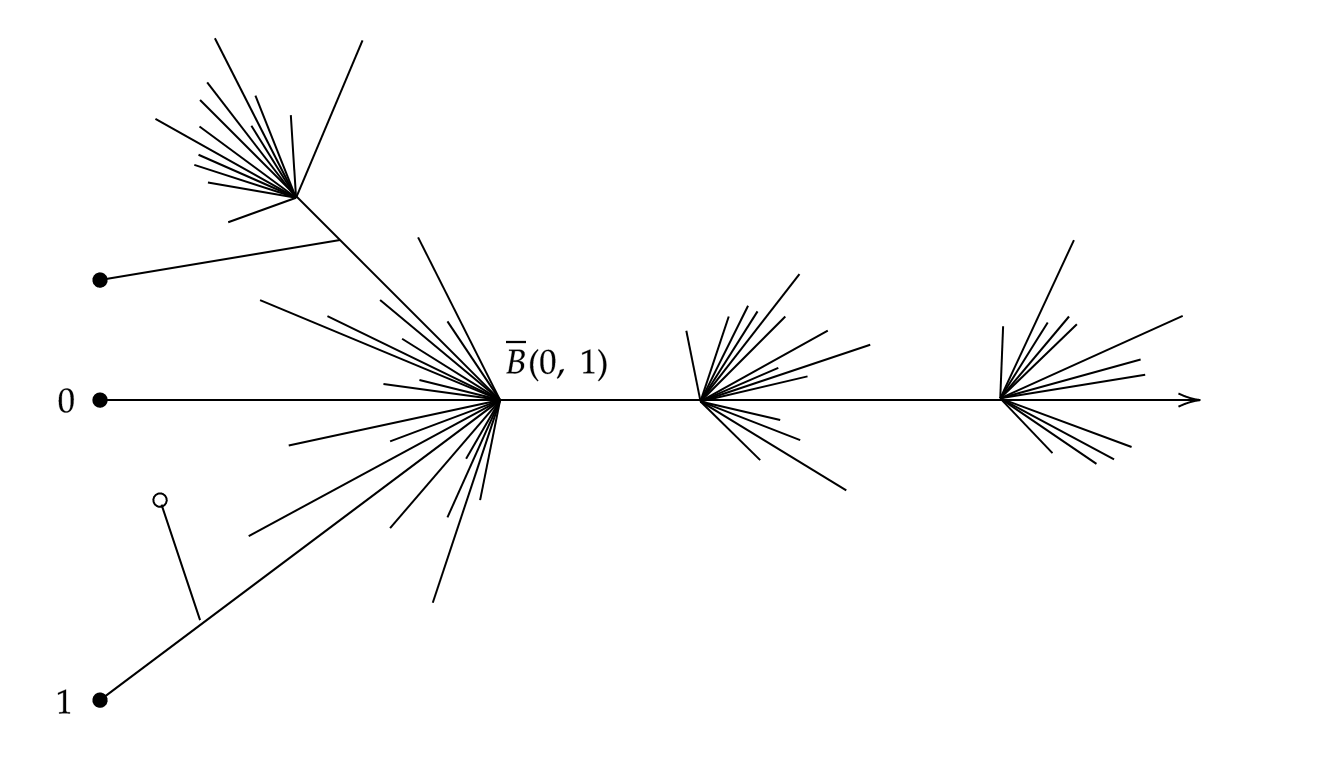
\includegraphics[width=0.7\textwidth]{Images/affineline.png}
    \caption{Visualisation of $\affline$}
    \label{fig:affline}
\end{figure}

Following the presentation in \parencite{bpr}, we now define some analytic domains in $\affline$ by using the fact that there is a continuous map $\sigma: \RR_{\geq 0} \to \affline$ mapping $r \mapsto \zeta_{0, r}$, which is a homeomorphism onto its image. 
We will refer to this image as the embedded real line. 
Then, $\sigma$ is a section of the map $\evt(x) = |T|_x$, and we find that these maps make the embedded real line into a strong deformation retract of $\affline$. 
Indeed, for any point $x \in \affline$, there is a point $\alpha := \sigma \circ \evt(x)$ lying on the embedded real line. 
By our earlier exposition, there is then a path $\gamma$ from $x$ to $\alpha$ parameterised by the unit interval. 
Hence, the map $F(x, t) = \gamma(t)$ is a homotopy satisfying the conditions of a strong deformation retract. 
These ideas will lead to the notion of the \textit{skeleton}, which will later become central to our study of $k$-analytic spaces.


We find that for any $I \subset \RR_{\geq 0}$, $\evt^{-1}(I)$ consists of the points which retract onto the points $\sigma(I)$. Then \cref{prop:diskmaxpoint} indicates that the closed (respectively, open) disk of radius $r \in |k^\times|$ can be visualised as $\evt^{-1}(I_r)$ where $I_r = [0, r]$ (respectively, $I_r = [0, r)$). Similarly, \parencite[\S 2.1]{bpr} we define the standard closed annulus $\mathbb{S}(a, b)$ of inner radius $|a|$ and outer radius $|b|$, for $0 < |a| \leq |b|$ and $a, b \in |k^{\times}|$ as the subset $\evt^{-1}([a, b])$, and when $a \neq b$, the standard open annulus as $\evt^{-1}((a, b))$. 
The closed annulus is affinoid, as it is identified with the spectrum of the following $k$-affinoid algebra:
\begin{align*}
k\{|a| \cdot T^{-1}, |b|^{-1} \cdot T\} & = \left\{ \sum_{i = -\infty}^{\infty} a_i T^i \; | \; |a_i| \cdot |a|^i \to 0 \; \text{as} \; i \to \infty, |a_i| \cdot |b|^i \to 0 \; \text{as} \; i \to -\infty \right\}.
\end{align*}

The norm on this algebra is given by 
\[
    \left\vert \sum_{n = -\infty}^{\infty} a_n T^n \right\vert = \max \{ |a_n| \cdot |a|^n, |a_n| \cdot |b|^n \}.
\]


\begin{figure}[!ht]
    \centering
    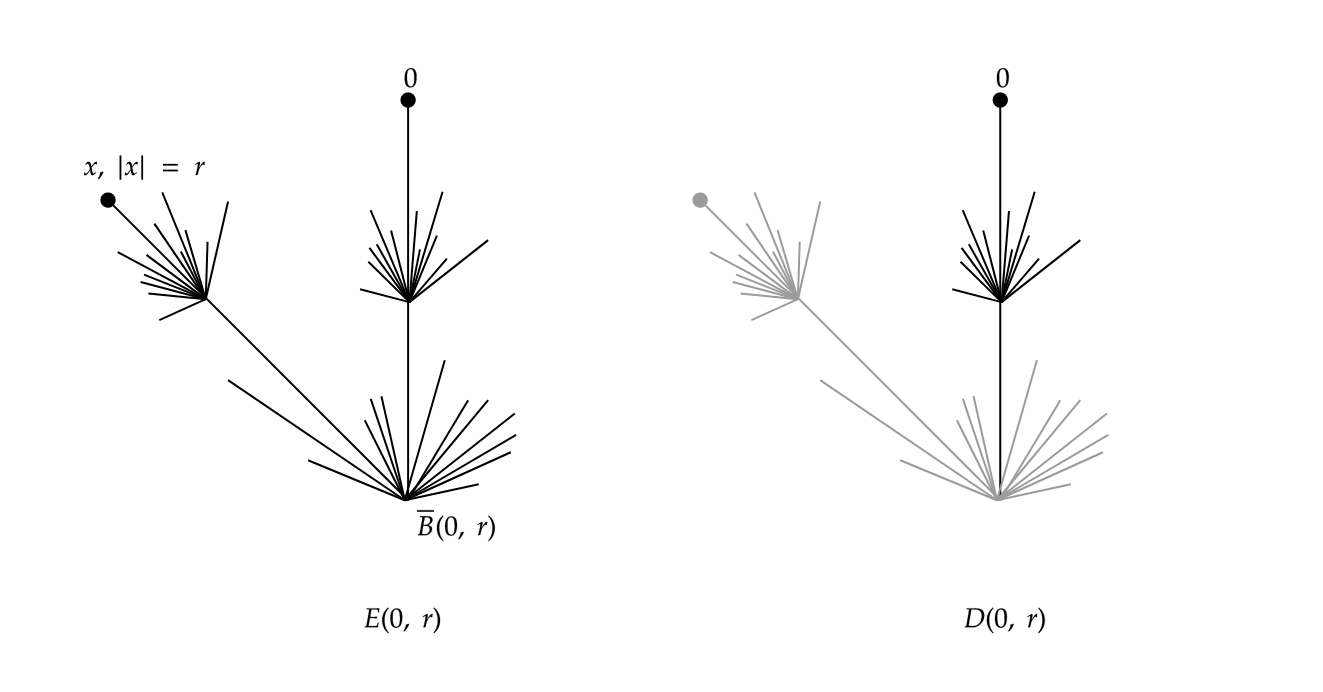
\includegraphics[width=0.8\textwidth]{Images/disks.png}
    \caption{Closed (left) and open (right) Berkovich disks}
    \label{fig:disks}
\end{figure}

\subsection{Gluing $k$-Analytic Spaces}

As is the case for topological and algebraic spaces, we may glue $k$-analytic spaces under appropriate conditions. A family of $k$-analytic spaces $\{X_i\}_{i \in I}$ gives gluing data if for each pair $i, j \in I$ there are analytic domains $X_{ij} \subset X_i, X_{ji} \subset X_j$ with an isomorphism $\mu_{ij}: X_{ij} \to X_{ji}$ satisfying the conditions:
\begin{enumerate}
    \item $X_{ii} = X_i$ and $\mu_{ii} = id$;
    \item $\mu_{ij}(X_{ij} \cap X_{ik}) = X_{ji} \cap X_{jk}$;
    \item $\mu_{ik} = \mu_{jk} \circ \mu_{ik}$.
\end{enumerate}

\begin{theorem} \label{gluing} \parencite[Prop. 1.3.3]{berk93}
    Let $\{X_i\}_{i \in I}$ be $k$-analytic gluing data. Suppose that one of the two following conditions holds.
    \begin{enumerate}
        \item Each $X_{ij} \subset X_i$ is open.
        \item Each $X_{ij} \subset X_i$ is closed, and for each $i \in I$, $X_{ij} \neq \emptyset$ for only finitely many $j \in I$.
    \end{enumerate}
    In each case, there exists a $k$-analytic space $X$ such that:
    \begin{enumerate}
        \item For each $i \in I$ there exists a morphism $\phi_i: X_i \to X$ making $X_i$ into an analytic domain in $X$.
        \item The images $\phi_i(X_i)$ cover $X$.
        \item $\phi_i(X_{ij}) = \phi_i(X_i) \cap \phi_j(X_j)$.
        \item $\phi_i(X_{ij}) = (\phi_j \circ \mu_{ij})(X_{ij})$
    \end{enumerate}
\end{theorem}

The proof of this is omitted and may be found in \textit{loc. cit.} Instead, we consider the analytic projective line to exemplify both types of gluing \parencite[Exercise 4.1.4.2]{temk}. 
Using the first kind of gluing, we may form $\projlinean$ using affine opens. Let $X_1 = X_2 = \affline$ and $X_{12} = X_{21} = {\{ x \in \affline \; | \; |T|_x \neq 0 \}}$. An isomorphism of analytic domains is then induced by the map $T \mapsto T^{-1}$. Concretely, it maps a seminorm $\snormx$ to the seminorm $|\cdot|_{1/x}$, where:
\[
    |a_nT^n + \cdots a_0|_{1/x} := |T|_{x}^{-n} \cdot |a_n + \cdots + a_0T^n|_x
\]
Using the second kind of gluing, $\projlinean$ may instead be constructed by gluing the unit disks $X_1 = X_2 = \berkspec{k\{T\}}$ along the closed analytic domains $X_{12} = X_{21} = {\berkspec{k\{T, T^{-1}\}}} = \{ x \; | \; |T|_x = 1 \}$. 
Similarly to the previous case, the isomorphism is induced by the homomorphism $k\{T, T^{-1}\} \to k\{T, T^{-1}\}$ mapping $T \mapsto T^{-1}$. 
This construction mirrors that of forming the Riemann sphere by gluing two closed disks along their boundaries. We will delay the proof that these two constructions are isomorphic until we have covered the notion of formal models; instead, we provide some pictorial intuition in \cref{fig:projline}. 
The left image visualises the gluing of the two affine lines while the right image shows the gluing of the unit disks; the analytic domains which are identified by the gluing are indicated with dashed lines.

\begin{figure}[!ht]
    \centering
    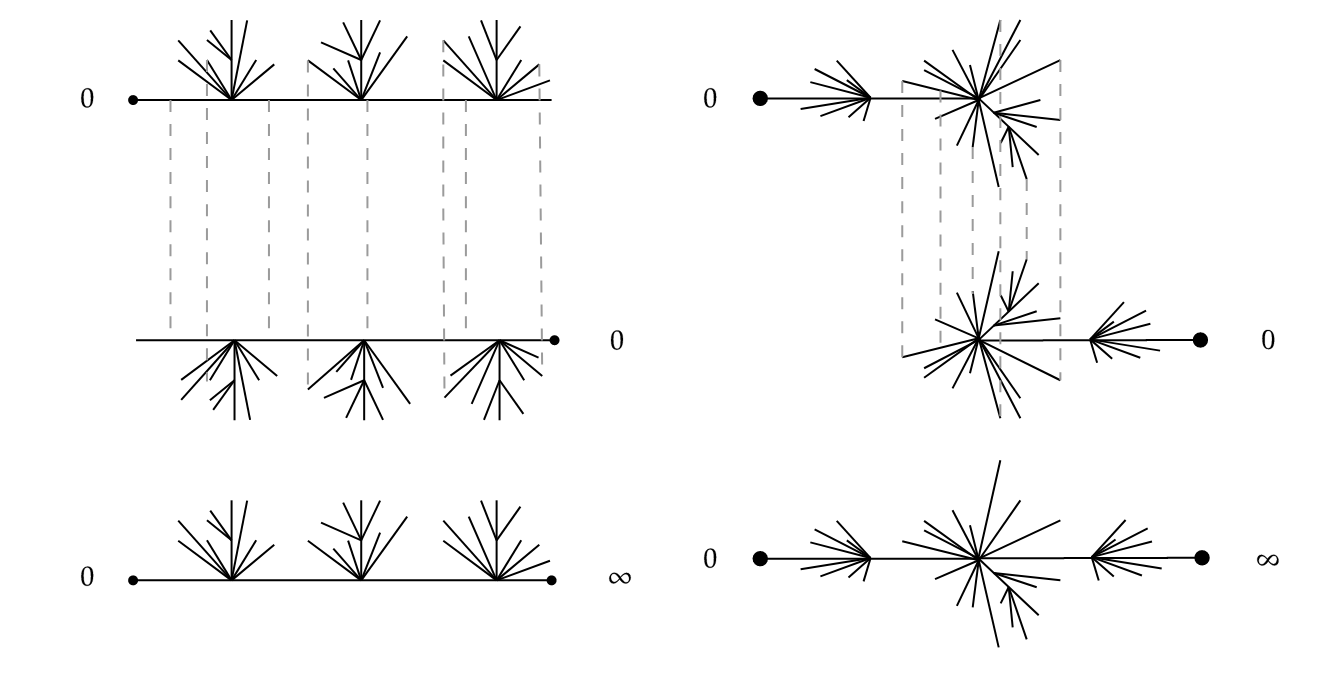
\includegraphics[width=0.8\textwidth]{Images/projspace.png}
    \caption{Two possible methods of constructing $\projlinean$}
    \label{fig:projline}
\end{figure}

The gluing procedure we have described may not, in general, result in a good $k$-analytic space.
For example, gluing two copies of the unit disk $\berkspeck{T}$ along the isomorphism given by $\berkspeck{T, T^{-1}} \cong \berkspeck{T, T^{-1}}$ given by the identity map.
In this case, we obtain the closed unit disk with a `doubled open unit disk.'
The point corresponding to $\zeta_{0, 1}$ does not admit an affinoid neighbourhood in this space.

\subsection{The Analytification Functor}

Similarly to the analytification of a complex variety, we can form the analytification of a variety over the non-Archimedean field $k$. The process is described following the presentation in \parencite[\S 3.4]{berk1}. The aim of the procedure is to assign to any scheme locally of finite type $X$ a $k$-analytic space $\anl{X}$ and a map $\iota: \anl{X} \to X$ of locally ringed spaces with the following universal property: if $Z$ is any $k$-analytic space and $\phi: Z \to X$ is a map of locally ringed spaces, then there is a unique factorization $\tilde{\phi}: Z \to \anl{X}$ through $\iota$, where $\tilde{\phi}$ is a map of $k$-analytic spaces.

For the scheme $\spec k[T_1, \dots, T_n]$, the analytification is the space $\mathbb{A}^{n, \text{an}}_{k}$ described previously. The map $\iota: \affnspace \to \mathbb{A}^{n}_{k}$ is given by mapping a seminorm to the point corresponding to the prime ideal given by its kernel.
Now assume we have obtained the analytification of $X$ and $Y \subset X$ is an open subscheme. Then we set $\anl{Y} = \iota^{-1}(Y) \subset \anl{X}$. 
If $Y \subset X$ is a closed subscheme defined by a coherent $\sheaf_{X}$ ideal $\mathfrak{J}$, then $\anl{Y}$ is the closed subspace cut out by $\mathfrak{J}\sheaf_{\anl X}$, which is a coherent $\sheaf_{\anl X}$ ideal. 
Finally, for any scheme $X$ locally of finite type covered by open affine subschemes $\{X_i\}_{i \in I}$, we may glue together the analytifications $X_i$ since by the universal property, the gluing data of the schemes induces gluing data for the analytifications. 
The canonical map of locally ringed spaces $\iota: \anl{X} \to X$ has the property that the induced homomorphism of stalks $\iota_x: \sheaf_{X, \pi(x)} \to \sheaf_{\anl{X}, x}$ is local and flat \parencite[Theorem 3.4.1]{berk1}. The proof that the constructions satisfy the desired universal property is omitted.

To exemplify the analytification functor, we now work out some explicit examples. Firstly, we note that the above construction applied to $\mathbb{P}^{1}_{k}$ yields the space $\projlinean$ constructed as the gluing of two analytic affine lines, justifying the notation.

Next, let $X$ be $n$-dimensional affine space and let $Y$ be the closed subscheme cut out by the ideal generated by some function $f \in k[T_1, \dots, T_n]$. Denote the corresponding $\sheaf_{X}$-ideal by $\mathfrak{J}$ and the $\sheaf_{\anl X}$-ideal corresponding to $\anl Y$ by $\anl{\mathfrak{J}}$. The space $\anl{Y}$ is identified, by construction, with the set of points 
\[
\{ x \in \mathbb{A}^{n, \text{an}}_{k} \; \vert \; \forall g \in \anl{\mathfrak{J}_{x}}, \; \; g(x) = 0 \}
\] 
where $g(x)$ denotes the image of $g$ in the residue field $\kappa(x) := \sheaf_{\mathbb{A}^{n, \text{an}}, x}/\mathfrak{m}_{x}$. Hence, it may be described as the points $x$ where $\anl{\mathfrak{J}_{x}} \subset \mathfrak{m}_{x}$. Denoting by $f_x := \pi_{x}(f_{\pi(x)})$ the image of the germ of $f$ at $\pi(x)$ under $\pi_x$ we find:
\[
\anl{\mathfrak{J}_x} \subset \mathfrak{m}_x
\iff \mathfrak{J}_{\pi(x)} \sheaf_{\anl X, x} \subset \mathfrak{m}_{\anl X, x} 
\iff f_x \in \mathfrak{m}_{\anl X, x}  
\]
Now, since $\pi_x$ is local:
\begin{align*}
    f_x \in \mathfrak{m}_{\anl X, x}
    \iff f_{\pi(x)} \in \mathfrak{m}_{X, \pi(x)}
    \iff f(x) = 0 \in \resfield 
    \iff |f|_x = 0
\end{align*}
Therefore, $\anl Y$ is the set of points of $\anl X = \mathbb{A}^{n, \text{an}}$ that one might intuitively expect - namely, the seminorms $|\cdot|_x$ on $k[T_1, \dots, T_n]$ such that $|f|_x = 0$.

Another example which will appear often is the analytification of the algebraic torus. As a scheme, we have that $\mathbb{G}_{m, k} = \spec k[T, T^{-1}]$, which is an open subscheme of the affine line. Hence, the analytification is given by the set of points $x \in \affline$ such that the kernel is not the ideal $(T)$, so $\anl{\mathbb{G}_{m, k}} \subset \affline$ consists of every point except for the type I point $\zeta_{0, 0}$.

The analytification preserves several desirable properties, which we state without proof (see \parencite[Theorem 3.4.8]{berk1}).
We will use these facts freely in the sequel.
Let $X$ be a scheme of locally finite type over $k$. 
Then:
\begin{enumerate}
    \item $X$ is separated if and only if $\anl{X}$ is Hausdorff;
    \item $X$ is proper if and only if $\anl{X}$ is Hausdorff and compact;
    \item $X$ is connected if and only if $\anl{X}$ is arcwise connected;
    \item the dimension of $X$ equals the topological dimension of $\anl{X}$.
\end{enumerate}

The full theory of Berkovich spaces is a deep and rich field of study of which we have seen only a small glimpse.
Equipped with our understanding of analytic spaces, we now broaden our investigations from the affine line to more general analytic curves.
